%!TeX root = note
\documentclass[main.tex]{subfiles}

\begin{document}
    \chapter{Circuit Principle}

    \section{MOSFET load switch}
    \justify
    In this section, the switching operation of a MOSFET is discussed
    \begin{enumerate}
        \item MOSFET switching principle.
        \item Gate charge.
        \item Safe Operating Area.
        \item Other parameters.
    \end{enumerate}

    \pagebreak
    \subsection{MOSFET basic switching circuit}

    \justify
    For the N-channel MOSFET to be  "switched on" (in triode or saturation region), the $V_{gs} > V_{th}$ with Gate-Source threshold voltage $V_{th} > 0$. A typical configuration of N-channel MOSFET switch is shown in Figure \ref{fig:NMOS_lowside_switch}. The PNP allows for the use small current switch signal (MCU, op-amp, etc.). The operation principle of the said circuit is as follows:

    \begin{itemize}
        \item To fully switch the N-channel MOSFET $M1$ on (saturation), the Gate voltage $V_{gs}$ must be greater than $V_{ds}-V_{th}$. Because the Source terminal is connected to Ground, the Gate can be connected directly to $V_{in}$ to turn on the MOSFET.
        \item When signal $V_s=0V$, the PNP transistor $Q1$ conducts, the Gate terminal is pulled down with $R2$, $M1$ is turned off. 
        \item When signal $V_s=5V$, $Q1$ stops conducting, the Gate terminal is pulled up with $R_{gate}$, $M1$ is turned on. 
        \item Because the load is an RC network, $M1$ should be turned on at a slower rate than turning off to reduce inrush current.
        \item The Zener diode $D1$ connected across the Source-Gate of $M1$ clamps the voltage at the diode zener breakdown voltage which is below the specified maximum $V_{gs}$

    \end{itemize}

    \begin{figure}[!h]
        \centerline{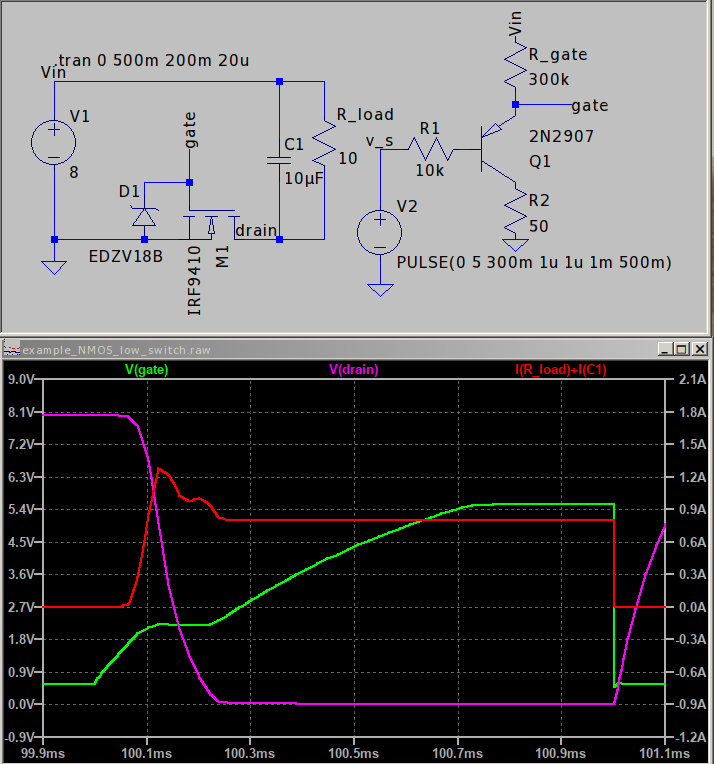
\includegraphics[scale=0.4]{media/example_NMOS_low_switch.png}}
        \caption{Transient analysis of turning on a MOSFET.}
        \label{fig:NMOS_lowside_switch}
    \end{figure}

    \pagebreak 
    \justify
    In the aforementioned configuration, the N-channel MOSFET's Source terminal is connected closer to ground than the load, $M1$ is called a \textbf{Low-side Switch}. Similarly, for the P-channel MOSFET whose "switched on" condition is $V_{gs} < V_{ds}-V_{th}$ with $V_{th} < 0$, the MOSFET is connected closer to $V_{in}$ than the load, thus, it is called a \textbf{High-side Switch}. An example circuit is shown in Figure \ref{fig:gate_charge_curve_2}. In this circuit, the gate is charged with a ideal power supply. blah

    \begin{figure}[!h]
        \centerline{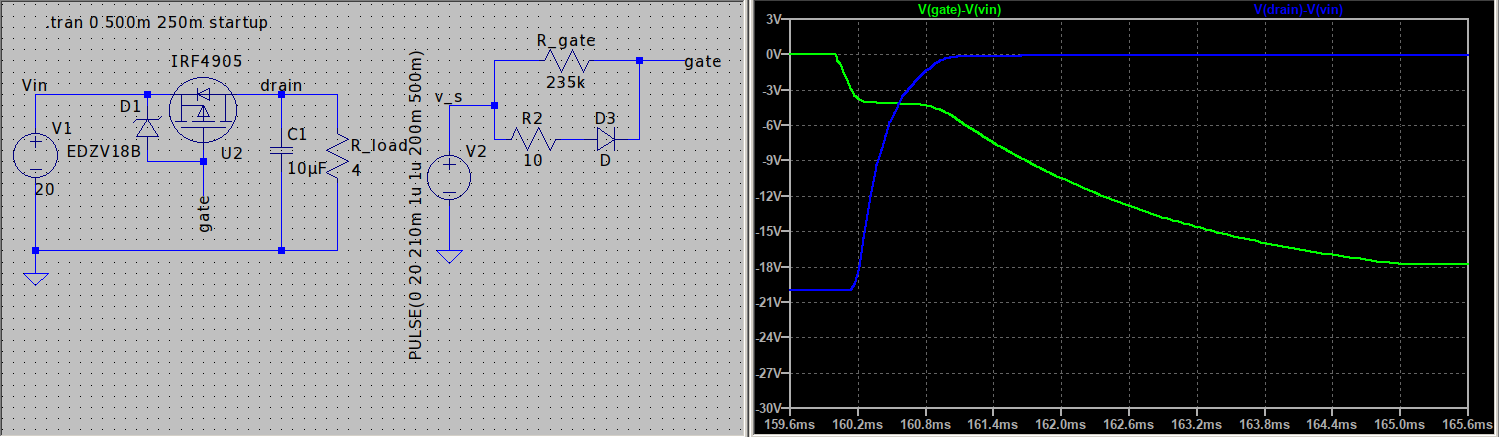
\includegraphics[width=\linewidth, height=0.5\linewidth]{media/gate_charge_curve_2.png}}
        \caption{Transient analysis of turning on a P-channel MOSFET}
        \label{fig:gate_charge_curve_2}
    \end{figure}

    \pagebreak
    \subsection{Type of load switch}
    \justify
    In load switching application, high-side switching is more preferable due to having no ground offset (ground loop). In a circuit exhibiting ground loop, the load is not connected directly to the ground of the power supply which can lead to distortion in signal transmission. The offset voltage is calculated by $\Delta V_\text{GND} = -I_d \cdot R_{ds}$ showing that $\Delta V_\text{GND}$ varied, and, thus, not desirable in electronics system. 
    
    \justify
    The use of P-channel MOSFET for this configuration has been discussed previously, and shown to be straight forward. However, to adopt a N-channel MOSFET is more complicated and requires the following extra design steps from the example circuit of Figure \ref{fig:gate_charge_curve_2}:
    \begin{itemize} 
        \item The source terminal of the N-channel MOSFET is connected to the positive terminal $V_{in}$ of the power supply. 
        \item As discussed in previously, $V_g$ must then be driven several voltages higher than $V_s = V_{in}$. This can be achieved by either a boost converter or a charge pump circuit \cite{InfineonNMOSHighDrive}, thus, increasing the complexity and component counts.
    \end{itemize}
    \subsection{On resistance $R_{ds}$}
    N-channel MOSFET exhibits lower $R_{ds}$ than that of P-channel MOSFET due to packing density. It is possible to parallel two or more P-channel MOSFETs to reduce the total on resistance $R_{\sum ds}$. However, the designer has to take into account devices' parameters mismatch. An application note from Infineon and Texas Instruments \cite{InfineonParallelMOS} details the effects and solutions of each mismatches, suitable for paralleling up to 4 MOSFETs. However, \cite{MOSFET_parallel_low_power} shows that for low power application, the parameter mismatches is not as detrimental as high power application.
    
    \pagebreak
    \subsection{Gate Charge}

    \justify
    In Figure \ref{fig:gate_charge_curve_2}, during a turn-on event, it can be divided into four main intervals. These intervals are shown in Figure \ref{fig:gate_charge_curve_details}.
    \begin{enumerate}
        \item $t_0 \rightarrow t_1$: $V_{gs}$ drops to approximately $V_{th}$. At this voltage, the MOSFET enters its ohmic/linear region and starts to conduct $I_d$.
        \item $t_1 \rightarrow t_2$: $V_{gs}$ drops to $V_{gs,miller}$. At this voltage, the MOSFET is still in its linear region.
        \item $t_2 \rightarrow t_3$: While $V_{gs}$ maintains at $V_{gs,miller}$- \textbf{Miller plateau}, $V_{ds}$ starts to increases rapidly, allowing $I_d$ to gradually increases. $V_{ds}$ reaches its turn-on voltage $R_{ds}(on)\cdot I_d$ of a few $mV$, and the MOSFET enters its saturation region.
        \item $t_3 \rightarrow t_4$: In the saturation region, $V_{gs}$ starts increasing to $V_{signal}$. However, $V_{gs}$ is clamped at $D1$'s zener voltage. 
    \end{enumerate}

    \begin{figure}[!h]
        \centering
        \begin{minipage}{.5\textwidth}
          \centering
          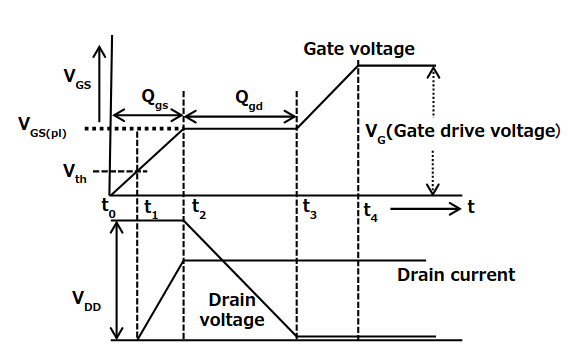
\includegraphics[width=\linewidth]{media/gate_charge_curve_details.png}
          \captionof{figure}{Typical gate charge curve.}
          \label{fig:gate_charge_curve_details}
        \end{minipage}%
        \begin{minipage}{.5\textwidth}
          \centering
          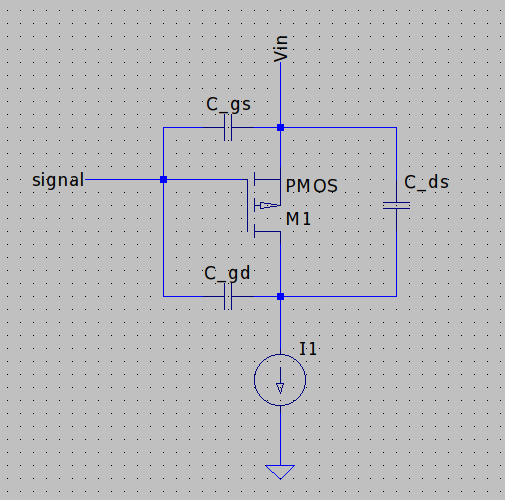
\includegraphics[width=0.8\linewidth]{media/MOSFET_parasitic_cap.png}
          \captionof{figure}{Model of MOSFET parasitic capacitance.}
          \label{fig:MOSFET_parasitic_cap}
        \end{minipage}
    \end{figure}

    \justify
    This phenomenon is due to the parisitic capacitance modeled in Figure \ref{fig:MOSFET_parasitic_cap}, which has to be charged partially before the MOSFET enters its saturation region. In a MOSFET datasheet, this charge value is reflected by $C_{gs}$ and $C_{gd}$. In particular:

    \begin{itemize}
        \item $t_0 \rightarrow t_2$: During these periods, both $C_{gs}$ and $C_{gd}$ are charged in parallel via $R_{g}$ until $V_{gs} = V_{gs, miller}$, thus, the charging time and the charge is defined by:
        \begin{equation}
            \Delta t_{0\rightarrow2}=R_{g}(C_{gs} +C_{gd})ln\left(\dfrac{V_{signal-source}}{V_{gs, miller}}\right)
        \end{equation}
        \begin{equation}
            Q_{0\rightarrow2}=(C_{gs} +C_{gd})\cdot (-V_{gs, miller})
        \end{equation}
        \item $t_2 \rightarrow t_3$: Voltage at Gate is maintained while $V_{ds}$ is decreases, meaning that $C_{gd}$ is being charged with a constant current flowing through $R_{g}$. Thus, the following equation: 
        \begin{equation}
            \dfrac{\delta V_{ds}}{\delta t}=\dfrac{1}{C_{gd}}\cdot\dfrac{V_{signal-source} - V_{gs,miller}}{R_{g}} \Rightarrow \Delta V_{ds} = \dfrac{V_{signal-source} - V_{gs,miller}}{R_{g}C_{gd}}\cdot \Delta t_{2\rightarrow3}
        \end{equation}
        \begin{equation}
            Q_{2\rightarrow3}= \left| \dfrac{V_{signal-source} - V_{gs,miller}}{R_{g}} \right|\cdot \Delta t_{2\rightarrow3} 
        \end{equation}
        Ideally, in saturation region, $V_{ds} = 0V \Rightarrow \Delta V_{ds} = -V_{in}$. Therefore:
        \begin{equation}
            \Delta t_{2\rightarrow3}=\dfrac{V_{signal-source}}{V_{signal-source} - V_{gs,miller}}\cdot R_{g}C_{gd}
        \end{equation}
        \begin{equation}
            Q_{2\rightarrow3}= -V_{signal-source}\cdot C_{gd}
        \end{equation}
        \item $t_3 \rightarrow t_4$: Similar to $\Delta t_{0\&2}$, $C_{gs}$ and $C_{gd}$ are charged in parallel via $R_{g}$ until $V_{g} = V_{signal}$.
    \end{itemize}

    \justify
    In this project's application, which does not involve high speed switching, only the interval $t_0 \rightarrow t_3$ is concerned (from turn-off and saturation region of the MOSFET). Thus, the total turn-on time $T_{on}$ and turn-on charge $Q_{on}$ is:

    \begin{equation} 
        T_{on} = R_{g}(C_{gs} +C_{gd})ln\left(\dfrac{V_{signal-source}}{V_{gs, miller}}\right) + \dfrac{V_{signal-source}}{V_{gs,miller}}R_{g}C_{gd}
    \end{equation}

    \begin{equation}
        Q_{on} = -[(C_{gs} +C_{gd})\cdot V_{gs, miller} - V_{signal-source}\cdot C_{gd}]
    \end{equation}

    \justify
    In a MOSFET datasheet, the value of $C_{gs}$ and $C_{gd}$ are shown in terms of input capacitance $C_{iss}$ and reverse transfer capacitance $C_{rss}$ which are plotted in the datasheet such as Figure \ref{fig:typical_capacitance_plot}. From the plot, the differnce between $C_{iss}$ and $C_{rss}$ are approximately constant, indicating that $C_{gs}$ is constant, while $C_{gd}$ is non-linear and voltage dependent.

    \begin{figure}[!h]
        \centerline{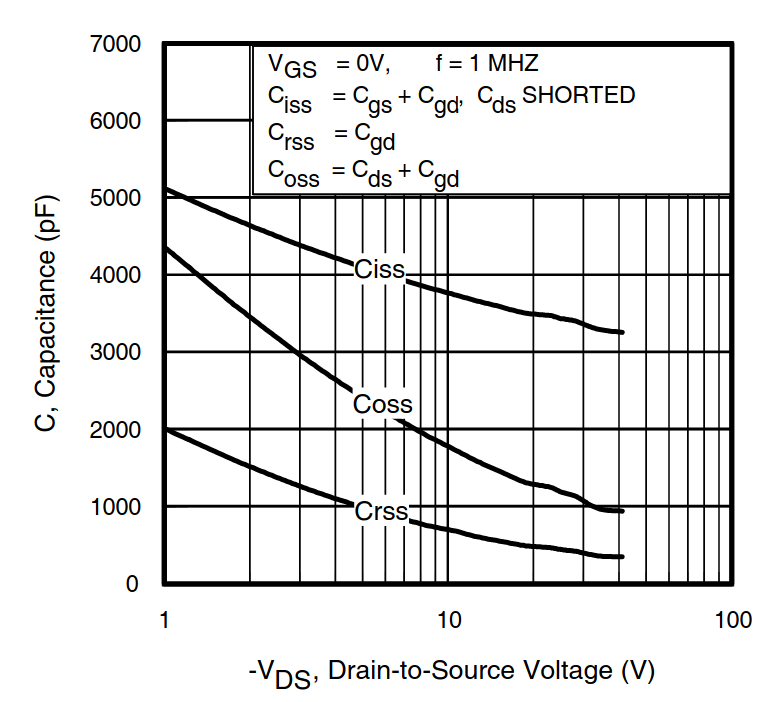
\includegraphics[scale=0.25]{media/typical_capacitance_plot.png}}
        \caption{Typical capacitance vs. Drain-Source voltage.}
        \label{fig:typical_capacitance_plot}
    \end{figure}

    \justify
    The calculations presented above are complex and cannot account for every turn-on scenarios because of the varying value of $C_{gd}$ dependent of $V_{in}$ and $V_{gs,miller}$ dependent of $I_{d}(\infty)$ (after fully switched on). The nonlinear function of $V_{gs,miller}(I_d)$ is shown in Equation \eqref{eq:estimated_miller_voltage_TI}. Furthermore, the charging of $C_{gd}$ and $C_{gs}$ is not continuously, causing plateau in $I_{g}$ curve similar to that of $V_{gs}$. Instead, a constant value of charge $\hat{Q}_{on}$ is used, and is estimated from the worst-case of the project's application. Equation \eqref{eq:estimated_on_charge} shows the estimated turn-on charge $\hat{Q}_{on}$.

    \begin{equation} \label{eq:estimated_miller_voltage_TI}
        V_{gs, miller} = V_{th} + \sqrt{\frac{I_{d}(\infty)}{K_n}}
    \end{equation}

    \begin{equation} \label{eq:estimated_on_charge}
        \hat{Q}_{on} = -[(C_{gs} +C_{gd}(V_{in}))\cdot V_{gs, miller} + V_{in}\cdot C_{gd}]
    \end{equation}

    \justify 
    Because in this project, the total maximum power is limited to $P_{max}=100W$, thus, $I_d(\infty) = P_{max}/V_{in}$. Equation \eqref{eq:estimated_on_charge} becomes a function of $V_{in}$:

    \begin{equation} \label{eq:estimated_on_charge_2}
        \hat{Q}_{on} = [C_{gs} +C_{gd}(V_{in})]\cdot \left(V_{th} + \sqrt{\dfrac{100W}{K_n\cdot V_{in}}} \right) + V_{in}\cdot C_{gd}(V_{in})
    \end{equation}

    \justify
    The value $V_{th}$ and $K_n$ are unique to each MOSFET, as well as $C_{gd}$. From the example plot shown in Figure \ref{fig:typical_capacitance_plot}, $C_{gd}$ can be modeled as a function of $V_{in}$.

    \pagebreak
    \subsection{Safe Operating Area (SOA)}
    In a MOSFET's datasheet, the SOA of the device shows the limitation of the device's opreating range. As long as the desired application is well within the SOA, the device will, in all likelihood, not risk running into problems such as thermal runaway, material degradation, etc. A typical SOA plot of a P-channel MOSFET is shown in figure \ref{fig:typical_SOA_plot}. The SOA lies below the dashed boundary. The SOA is defined by graphing the device's performance in the circuit shown in figure \ref{fig:SOA_circuit}.

    \begin{figure}[!h]
        \centering
        \begin{minipage}{.5\textwidth}
          \centering
          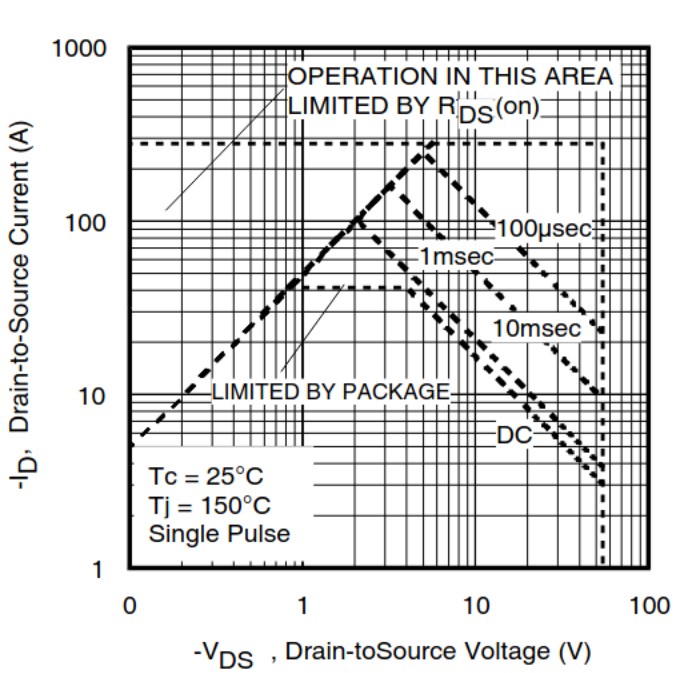
\includegraphics[width=0.8\linewidth]{media/typical_SOA_plot.png}
          \captionof{figure}{Typical MOSFET's SOA plot.}
          \label{fig:typical_SOA_plot}
        \end{minipage}%
        \begin{minipage}{.5\textwidth}
          \centering
          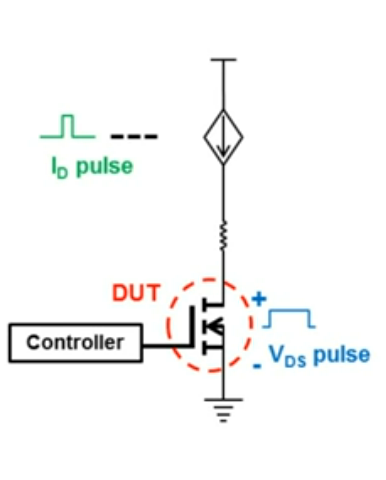
\includegraphics[width=0.8\linewidth]{media/SOA_circuit.png}
          \captionof{figure}{Typical MOSFET's setup for graphing SOA.}
          \label{fig:SOA_circuit}
        \end{minipage}
    \end{figure}

    \pagebreak
    \begin{figure}[!h]
        \centerline{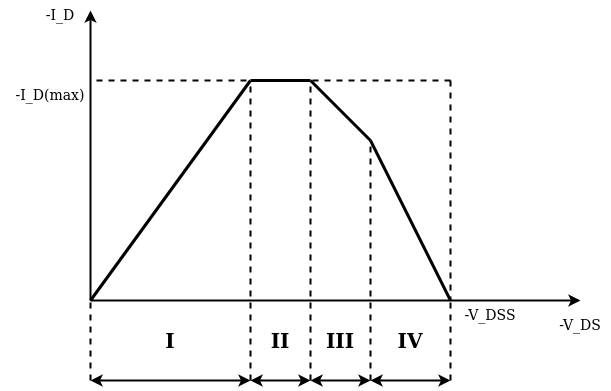
\includegraphics[scale=0.5]{media/SOA_regions.drawio.png}}
        \caption{Regions within a MOSFET's SOA.}
        \label{fig:SOA_regions}
    \end{figure}

    \justify
    The SOA can be divided into four regions shown in figure \ref{fig:SOA_regions}:
    \begin{enumerate}
        \item Region I: In this region, $-V_{ds}$ is determined purely by Ohm's law  $-V_{ds} = R_{ds}(\text{on})\cdot -I_d$ with $-I_d \leq -I_{d,\text{max}}$. Thus, region I spans from $-V_{ds} = 0$ to $-V_{ds} = \dfrac{-I_{d,\text{max}}}{R_{ds}(\text{on})}$.
        \item Region II: In this region, $-I_{d}$ is limited by $-I_{d,\text{max}}$ as a result of limitation of package, silicon and junction-to-ambient thermal impedance $R_{\theta J A}$. The power consumption $P=I_{d} * V_{ds}$ does not exceed the maximum rating. Thus, region II spans from $-V_{ds} = -I_{d,\text{max}} / R_{ds}(\text{on})$ to $-V_{ds} = \dfrac{P_\text{max}}{-I_{d,\text{max}}}$.
        \item Region III: In this region, the $-I_{d}$ is limited by $P_\text{max}$ or $-I_d = \dfrac{P_\text{max}}{-V_{ds}}$, hence, the negative coefficient observed from the plot.
        \item Region IV: The forth region is limited by thermal instability. 
    \end{enumerate}

    \justify
    Texas Instruments noted that region III and IV are difficult to define. In some device, the boundary of these two regions are seemingly unanimous. Hence, the application should be designed to operate well within the estimated regions defined in the datasheet. Besides region I, the other regions are soft-limited, meaning that operation outside of these regions does not guarantee immediate damage, however, the longevity of the devie is affected.

    \justify
    To ensure the operation of the MOSFET is well within the SOA, the following basic parameters of the device should be:

    \begin{enumerate}
        \item Drain-Source breakdown voltage $V_{dss}$ is at least 20\% higher than the operating voltage. 
        \item Maximum continuous Drain current $I_{d,\text{max}}$ is at least 20\% higher than the operating current.
        \item Low on resistance $R_{ds}$ satisfying the maximum dissipation power $P_{d}=R_{ds} \cdot I_{max}$ of the MOSFET.
    \end{enumerate}

    \pagebreak
    \subsection{IRF4905S}

    \justify
    As a load switch, the following parameters are basic to the selection process:
    \begin{itemize}
        \item Safe Operating Area is guaranteed.
        \item Parsitic capacitance $C_{gd}$ does not vary largely over the operating range.
    \end{itemize}

    \justify
    Between N-channel and P-channel MOSFET, within the same price range, $V_{ds}$ and $I_d$ are similar. The main differences are the switch type (high-side or low-side) and the $R_{ds}$. These differences are discussed in details in previous sections, and is summarized in Table \ref{table:MOSFET_channel_type}
    

    \begin{table}[!h]
        \centering
        \begin{tabular}{|m{0.15\linewidth}|m{0.4\linewidth}|m{0.4\linewidth}|}
        
        \hline
        & \textbf{P-channel MOSFET} &  \textbf{N-channel MOSFET} \\
        \hline
        \textbf{Switch type} & $V_{th} < 0V \Rightarrow$ High-side switch & 
        \begin{itemize}
            \item $V_{th} > 0V \Rightarrow $ Low-side switch leads to ground offset (ground loop) varied based on $R_{ds}$ and $I_{d}$ of MOSFET. Require a gate driver IC with integrated/discrete charge pump circuit to use as high-side switch.
        \end{itemize}
        \\
        \hline
        \textbf{Typical $R_{ds}$} & 
        \begin{itemize}
            \item High, in $100 m\ohm$ range $\Rightarrow$ High power loss. By paralleling, the on resistance is halved.
            \item Low $R_{ds}$ is more expensive than its N-channel counterpart.
        \end{itemize}
         
        & Low, in $m\ohm$ range $\Rightarrow$ Low power loss.
        \\
        
        \hline
        \end{tabular}
        \caption{Comparison of P-channel \& N-channel MOSFET}
        \label{table:MOSFET_channel_type}

    \end{table}    

    \justify
    Considering the advantages and disadvantages of the two type of MOSFET transistor, it is clear that using P-channel MOSFET as high-side switch is more advantageous in terms of components counts. Finally, the IRF4905S MOSFET is used because it has a suitable margin between its $V_{ds}$ and $I_{d}$ values and a low $R_{ds}$, making it ideal for this application. 

    \begin{figure}[!h]
        \centerline{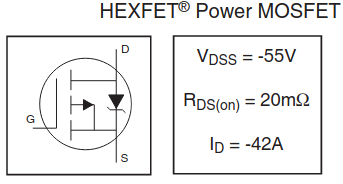
\includegraphics[scale=0.5]{media/IRF4905_key_parameters.png}}
        \caption{IRF4905 P-channel MOSFET key parameter \cite{IRF4905S}.}
        \label{fig:IRF4905S_param}
    \end{figure}    
    
    \section{MOSFET driver}
    
    \justify
    In our application which does not involve high speed switching, only $C_{gs}$ and $C_{gd}$ are of concern in transient analysis. For IRF4905S, the maximum total gate charge $Q_g$ is $180nC$. However, for the MOSFET to be in saturation mode, only the parasitic capacitors $C_{gs}$ and $C_{gd}$ needs to be charged. The gate charge curve follows a similar pattern shown in Figure \ref{fig:gate_charge_curve} extracted from the datasheet of IRF4905S. Simulating in LTspice, the curve of $V_gs$ and $I_g$ shows resemblance to the datasheet.

    \begin{figure}[!h]
        \centerline{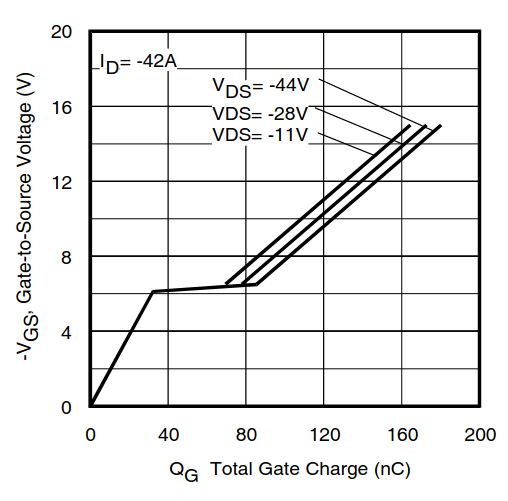
\includegraphics[scale=0.5]{media/gate_charge_curve.png}}
        \caption{IRF905S typical gate charge and Gate-to-Source voltage from datasheet.}
        \label{fig:gate_charge_curve}
    \end{figure}

    \begin{figure}[!h]
        \centerline{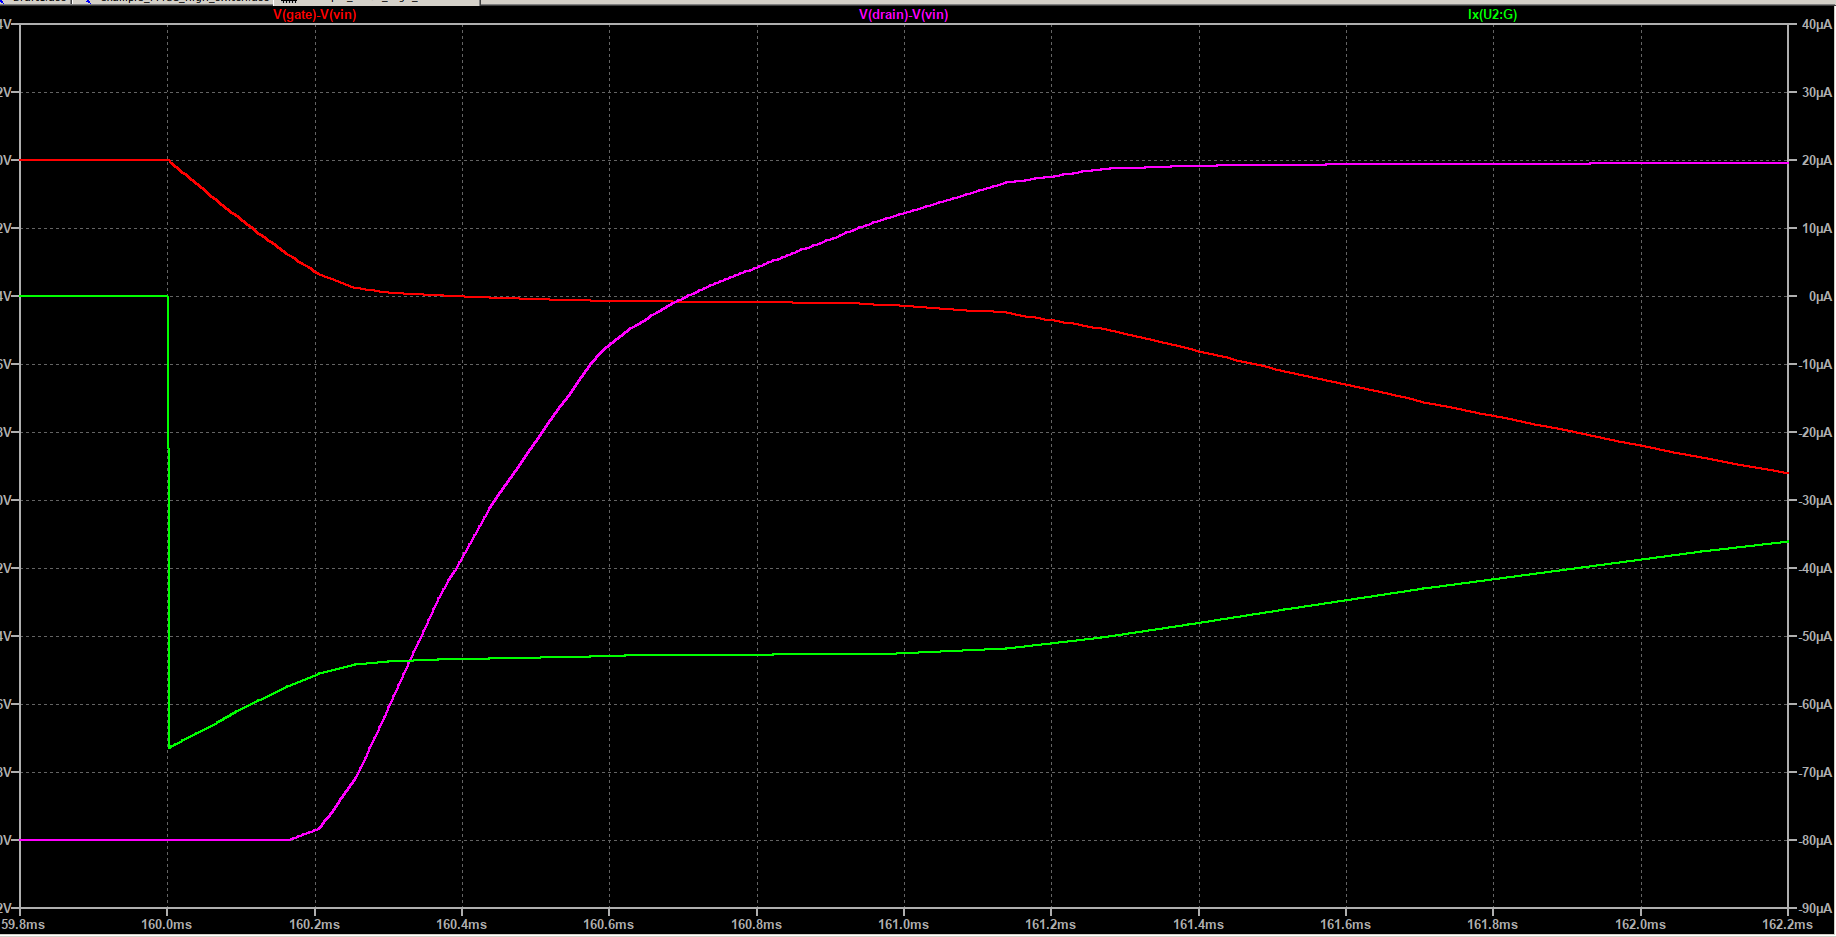
\includegraphics[width=\linewidth]{media/gate_charge_curve_3.png}}
        \caption{LTSpice simulation result for IRF905S gate charge and Gate-to-Source voltage.}
        \label{fig:gate_charge_curve}
    \end{figure}
    
    \justify
    For IRF4905S, the maximum total gate charge $Q_g$ is $180nC$, and the typical switching time $t_{sw}$ is approximately $100ns$. Then, the gate current needed to switch the MOSFET is $I_g = Q_g / t_{sw} = 1.8A$

    \justify
    Therefore, the 

    \justify
    
    \pagebreak

    \section{Overvoltage/Undervoltage Protection}

    \subsection{Overvoltage protection}

    \justify
    Reference schematic:

    \begin{figure}[!h]
        \centerline{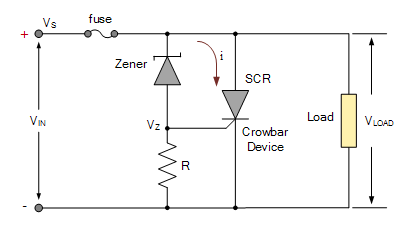
\includegraphics[scale=0.5]{media/Zener_Crowbar_OVP.png}}
        \caption{Electrical box arrangement overview.}
        \label{fig:enclosure_arrange}
    \end{figure}

    \subsection{Undervoltage Protection}
    
    \section{Isolation Protection}

    \section{Reverse Polarity Protection}

    \pagebreak

    \section{5V Rail}

    \subsection{Principle}
    \justify
    To supply power to the protection logic circuit and the MCU, a 5V rail is needed. The following are methods of creating such constant voltage rail from the main power supply:

    \begin{table}[!h]
        \centering
        \begin{tabular}{|m{0.1\linewidth}|m{0.45\linewidth}|m{0.45\linewidth}|}
        
        \hline
        & Linear voltage regulator & Switching voltage regulator \\
        \hline
        Principle & 

        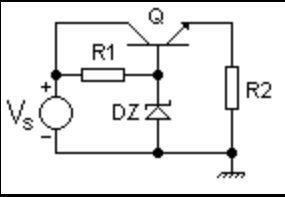
\includegraphics[width=0.45\textwidth]{media/series_regulator.png}
        The above figure illustrates a simple circuit of a linear voltage regulator. In this circuit, assuming a constant load, the voltage drop across $R_2$ is kept constant by biasing the transistor $Q$ with zener diode $DZ$. &

        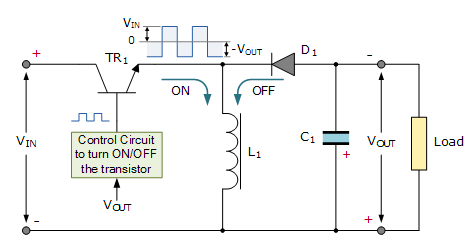
\includegraphics[width=0.45\textwidth]{media/inverting_switch_regulator.png}
        The above figure illustrates a simple switching voltage regulator. In this circuit, the close-open switching of the transistor stores and releases energy of the inductor which in turn charges the capacitor maintaining a constant voltage drop $V_{out}$ across the load. \\

        \hline
        Advantages & 

        \begin{itemize}
            \item Often comes as fixed output regulator which is suitable for digital logic ICs, and microcontrollers.
            \item Requires very few external components. In the case of fixed-output, only decouply capacitors at input and ouput are needed.
        \end{itemize} &
        
        \begin{itemize}
            \item Low power loss due to on(saturation)/off switching of the transistor leading to less conduction loss, allowing for higher current application.
            \item Can perform buck ($V_{out} < V_{in}$) and boost ($V_{out} > V_{in}$).
        \end{itemize} \\

        \hline
        Disadvantages & 

        \begin{itemize}
            \item High power loss. The transistor $Q$ is in its ohmic region due to the biasing of Base-Emitter region, thus, $I_{c} \approx I_{e}$. The power loss is approximated: \newline $P_{loss} = P_{in} - P_{out} = (V_{in} - V_{load}) \cdot I_{e}$.
            \item Can only perform voltage step-down ($V_{out} < V_{in}$).
        \end{itemize} &
        
        \begin{itemize}
            \item High component count.
            \item Switching noise due to continuous charge and discharge of inductor.
            \item Lower load regulation capability in comparison to linear voltage regulation. Load regulation are heavily dependent on the LC subcircuit. 
        \end{itemize}  \\

        \hline     
        \end{tabular}
        \caption{Comparison of linear and switching voltage regulator}
        \label{table:voltage_regulator_type}
    \end{table}

    \justify
    In summary, linear voltage regulator is suitable for low power application with limited input voltage range; while switching voltage regulator is suitable for medium power consumption with limited load regulation. In this project, the MCU consumes up to $0.5A$ during wireless transmission, and the undervoltage/overvoltage logic circuit consumes negligible current.

    \begin{itemize}
        \item Linear voltage regulator: Power loss is up to $P_{loss} = (V_{in,max} - 5V) \cdot 0.5A = (30V - 5V) \cdot 0.5A = 12.5W$ which is a efficiency of $\eta = \dfrac{2.5W}{15W} = 16.67\%$
        \item Switching voltage regulator: Switching noise and voltage ripple can negatively affect MCU's data transmission.
    \end{itemize}
    
    \justify
    To offset the disadvantages of the two type of voltage regulator, a hybrid where a switching voltage regulator first regulate the input voltage to $V_{out,sw}=10V$, and a linear voltage regulator regulate $V_{out,sw}$ down to $5V$ (the desired voltage). In this setup, the power loss of the linear regulator is $P_{loss} = (V_{out,sw} - 5V) \cdot 0.5A = (10V - 5V) \cdot 0.5A = 2.5W$; switching noise and ripple is reduced by the linear regulator. $V_{out,sw}$ can be further reduced, as long as the switching regulator allows, to reduce the power loss even further.

    \justify
    Because of the invering voltage of the switching regulator, the 5V rail created is -5V in reference to the supply voltage's ground. This is also applied to $V_{out,sw}$. The undervoltage/overvoltage logic circuit will be adjusted accordingly to compensate for the negative offset.

    \subsection{MC34063AD and L7805xx}

    \justify
    MC34063AD from Onsemi \cite{MC34063AD} is chosen for the construction of the switching regulator due to its few external component requirement. The IC has a built-in BJT load switch that can withstand 1.5A and shunt current sensing for overcurrent/short protection.

    \begin{figure}[!h]
        \centerline{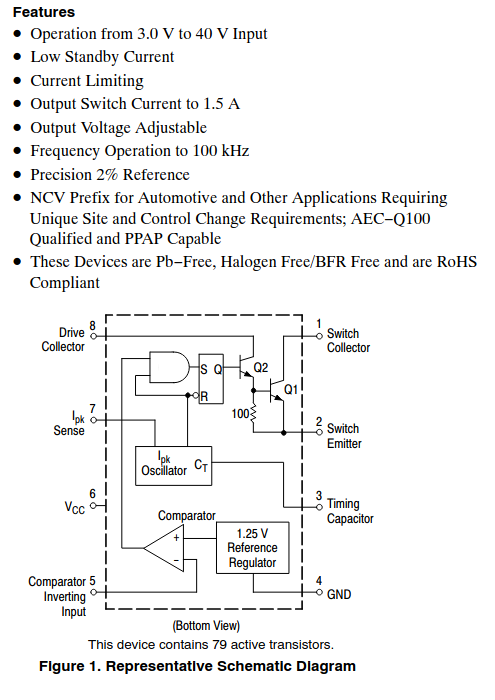
\includegraphics[scale=0.5]{media/MC34063AD_specs.png}}
        \caption{MC34063AD specifications.}
        \label{fig:MC34063AD_specs}
    \end{figure}

    \justify
    L7805xx series from STMicroelectronics \cite{L78} is chosen for the LDO.




    
    
\end{document}
